\chapter{Manifolds and Graphs}
\label{sec:manifold_and_graphs}
    
In this chapter, the connection between graphs and Graph Laplacian (GL) embedding to 
CT and cryo-EM is examined. 
First, some graph foundations are presented.
Then, GL and its embedding is introduced and the connection to CT and cryo-EM is illustrated.
Further, the term Graph Denoising is defined and last, some Graph Deep Learning approaches are presented.


\section{Graph Foundations}
Real world data is often in a graph structure, like social networks, citation networks,
protein interaction networks or a simple google search. 
If data is not available as a graph structure, a graph can be artificially constructed with k-NN or other methods.

\paragraph{Graph Learning:} 
Graph Learning got a lot of attention in recent years.
The idea is to learn graph information, such as topology or connections between nodes, to solve tasks.
Attention mechanisms are popular at the moment\cite{transformer} and the idea was derived to graphs as well \cite{GAT}.
It resumes to computing node features by using local information, therefore, the neighborhood of nodes is exploited.
Popular learning tasks are \textit{node classification} or \textit{link prediction}, where a model is learned from node and edge features 
as well as topology. The model can be used for prediction or classification on nodes or edges.
Another common task is \textit{community detection}, which aims to identify clusters of nodes within the input graph.
Further, graphs are highly favored for \textit{dimensionality-reduction}, where 
graph algorithms provide a helpful tool, as ordinary algorithms like principal component analysis fail to 
establish a meaningful dimensionality reduction.


\paragraph{Constructing Graphs for molecular-imaging:}
For a cryo-EM or CT observation, a graph can be constructed as well.
Every observation $y_i$ can be assigned to a node $v_i$, consequently $v_i \in \mathbb{R}^M$ and $|V|=N$.

To determine distance between two nodes, a distance measure needs to be defined.
For CT, it can be set up by using the $\ell2$-norm $\norm{y_i - y_j}$.
A cryo-EM distance measure is more challenging to setup, as projections are drawn with some random 3D rotation and projection.
It can happen that two observations are equivalent up to a 2D rotation. 
Consider a first observation $y_1$, which has no 3D rotation and 
a second observation $y_2$ with a rotation in x-y plane by 45°.
The two projections have a defined in-plane rotation $g$, such that $g \; y_1 = y_2$.
Therefore, a term of in-plane rotation is added to the $\ell2$-norm: $min_{g \in SO(1)}\norm{g \;y_i - y_j}$, 
which is inspired by \cite{multiDiffusionMaps}.


\section{Graph Laplacian \& Manifolds}
In the following section, the connection of GL and manifolds to CT and cryo-EM is established.

\subsection{Graph Laplacian}
GL is a matrix that represents a graph and can be used to find many important properties.
It is a very powerful tool and a good introduction can be found in \cite{tutorialSpectralClustering, SpectralGraphTheory}. 

GL is defined as follows: $L = D - A$, where $A$ is the adjacency matrix and $D$ the degree matrix (diagonal matrix with degree of nodes as entries).

\subsection{Graph Laplacian Embedding for CT and cryo-EM}
A basic introduction to GL embedding and how it can be computed is found in \ref{sec:manifolds}.
In this section, the connection to CT and cryo-EM is established.

For a given observation, a low-dimensional embedding can be computed by using the GL.
In the following, it will be observed how this embedding for CT looks like.
To be more precise, the second and third smallest eigenvectors of GL will be observed.
Shepp-Logan phantom is used again as an example for CT.
For Radon Transform, $\theta$ and $s$ are specified with $\theta \in \mathbb{R}^{500}$ as evenly spaced
between $[0, 2 \pi]$ and $dim(s) = 200$. 

In Figure~\ref{fig:clean_manifold}, embedding calculated from clean sinogram and $k=2$ can be seen.
It looks like a perfect circle and angles are in order. 
Further, noise was added to the sinogram to reach \snry 20 dB, 10 dB and 0 dB. 
Additionally, the embedding was computed with $k=6$ and illustrated in Figure~\ref{noisy_manifold_k6_snr20}, Figure~\ref{noisy_manifold_k6_snr10}
and Figure~\ref{noisy_manifold_k6_snr0} respectively.
For \snry 20 dB, a circle like object could be established and for \snry 10 dB it looks like a half circle. 

\textbf{TODO: adjust ticks for 0dB}

\begin{figure}[H]
    \captionsetup[subfigure]{justification=centering}
    \centering
    \begin{subfigure}[t]{0.25\textwidth}
        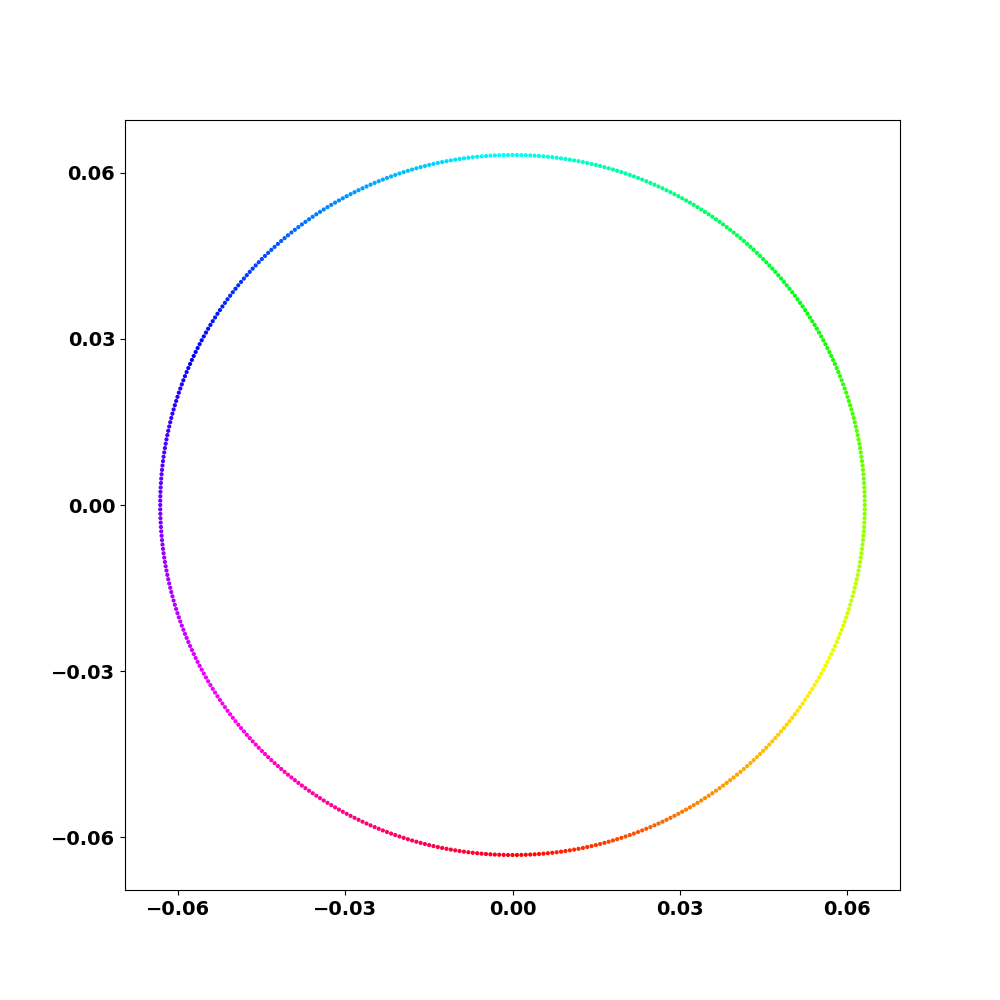
\includegraphics[width=\textwidth]{phaton_clean_manifold.png}
        \caption{Clean sinogram embedding with $k=2$}
        \label{fig:clean_manifold}
    \end{subfigure}\hfill
    \begin{subfigure}[t]{0.25\textwidth}
      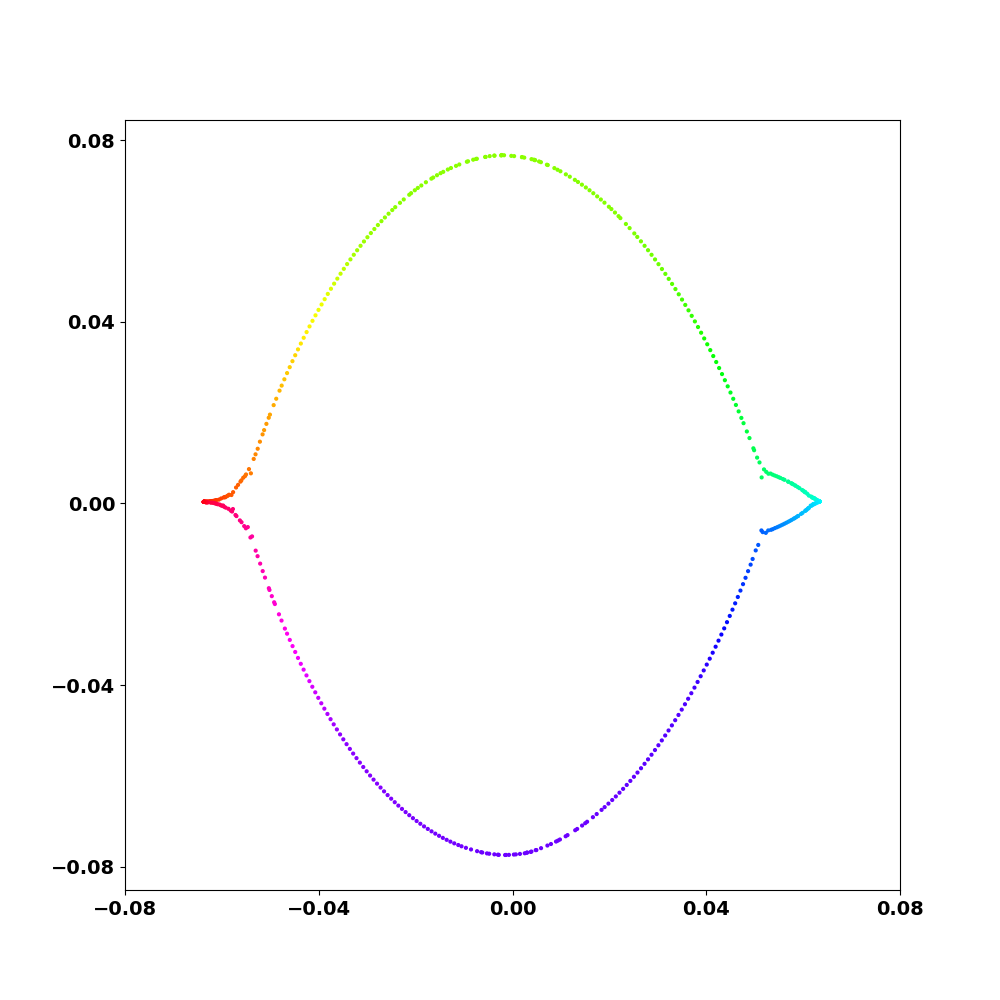
\includegraphics[width=\textwidth]{phaton_noisy_manifold_k6_snr20.png}
      \caption{GL embedding $k=6$ with \snry 20 dB}
      \label{fig:noisy_manifold_k6_snr20}
    \end{subfigure}\hfill
    \begin{subfigure}[t]{0.25\textwidth}
      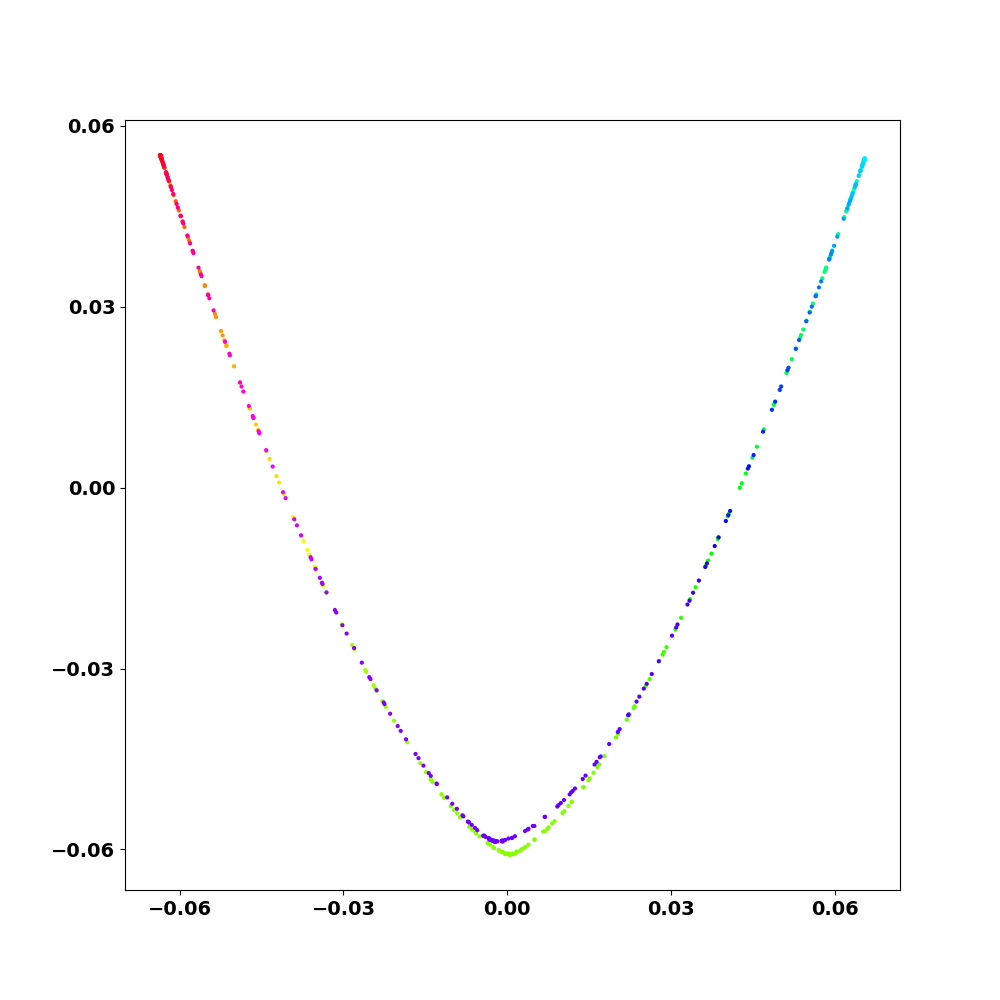
\includegraphics[width=\textwidth]{phaton_noisy_manifold_k6_snr10.png}
      \caption{GL embedding $k=6$ with \snry 10 dB}
      \label{fig:noisy_manifold_k6_snr10}
    \end{subfigure}\hfill
    \begin{subfigure}[t]{0.25\textwidth}
      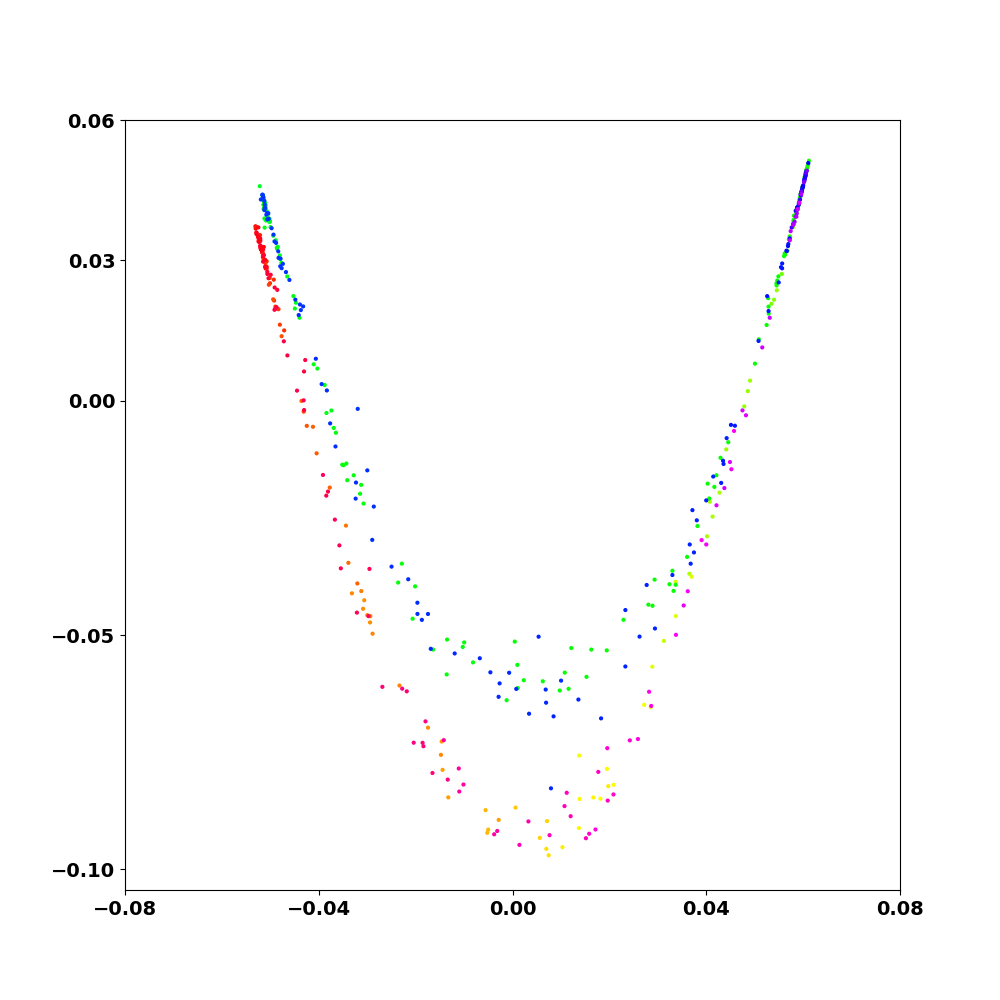
\includegraphics[width=\textwidth]{phaton_noisy_manifold_k6_snr0.png}
      \caption{GL embedding $k=6$ with \snry 0 dB}
      \label{fig:noisy_manifold_k6_snr0}
    \end{subfigure}
    \caption{Shepp-Logan phantom sinogram GL eigenvectors}
    \label{fig:phantom_manifolds}
  \end{figure}

\begin{tcolorbox}[colback=red!5!white,colframe=red!75!black]
    In the fields of CT and cryo-EM, underlying low-dimensional embedding from GL is well-defined for noiseless data.
    In 2D the underlying GL-manifold is a circle, whereas in 3D the GL-manifold is defined as a sphere.
    This fact can be exploited during learning.
\end{tcolorbox}

\paragraph{Tomography for unknown angles:}
But what can we use this embedding for?
It is defining a low-dimensional mapping from high-dimensional space.
In the case of CT and cryo-EM, this embedding approximates angles for observations.
Therefore, for (noisy) observations, angles can be approximated and reconstruction can be established even if angles are unknown.
The problem here is the quality of our embedding. As long as the computed embedding is a mapping to the circle (or sphere),
it should be reasonable to do reconstruction with.
In Figure~\ref{fig:phantom_fbp_unknown_angles} reconstruction with unknown angles is applied. Again, $k=6$
but \snry 20 dB and 0 dB are used. Clean reconstruction with approximated angles in Figure~\ref{fig:clean_reco_unknown} looks good, 
despite that there is an in-plane rotation of around 45 degrees. 
But even more moderate noise 20 dB, where the embedding almost looks like a circle (Figure~\ref{fig:noisy_manifold_k6_snr20})
the difference between reconstruction with known angles (Figure~\ref{fig:noisy_snr20_reco_known})
and unknown angles (Figure~\ref{fig:noisy_snr20_reco_unknown}) is pretty big.
For 0 dB, already with known angles (Figure~\ref{fig:noisy_snr0_reco_known}), reconstruction fails and with unknown angles barely anything from
original Shepp-Logan phantom can be determined  (Figure~\ref{fig:noisy_snr0_reco_unknown}).

\begin{figure}[H]
    \captionsetup[subfigure]{justification=centering}
    \centering
    \begin{subfigure}[t]{0.3\textwidth}
        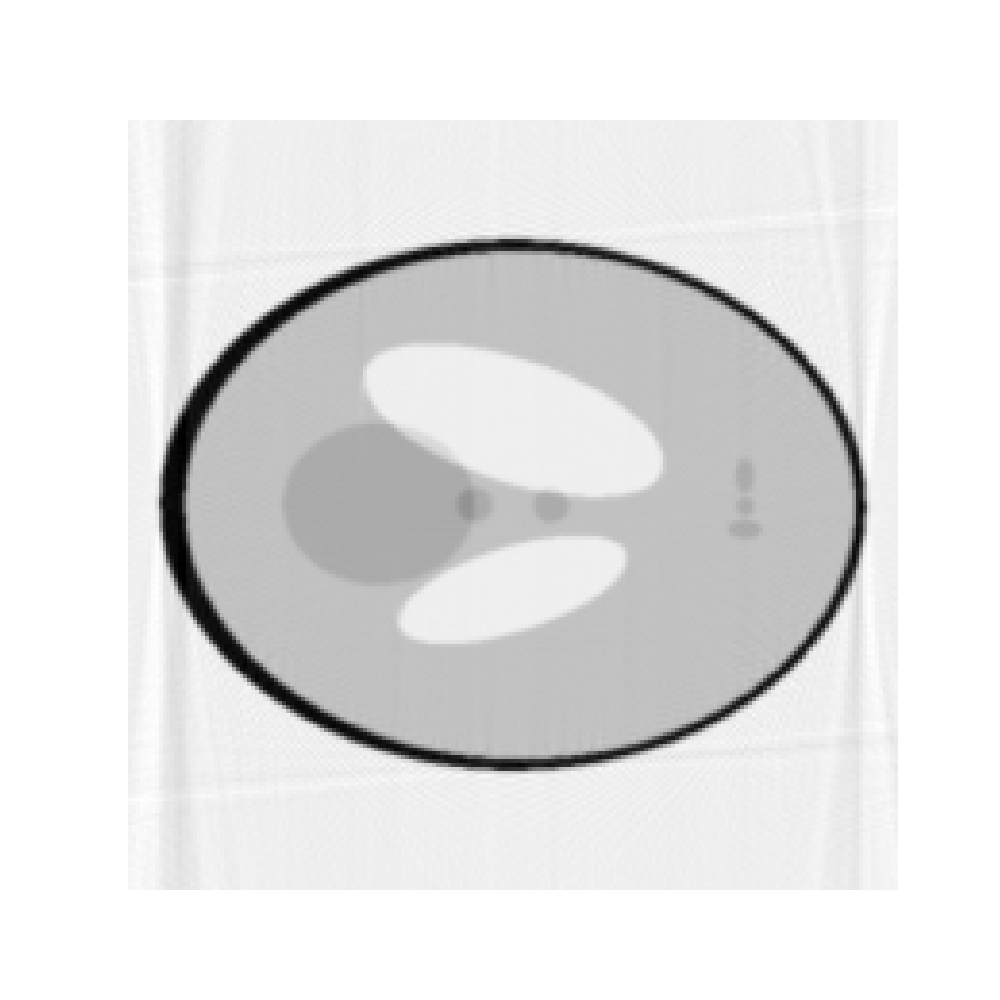
\includegraphics[width=\textwidth]{fbp_phantom_clean_unknown_angles.png}
        \caption{Clean sinogram reconstruction from GL estimated angles.}
        \label{fig:clean_reco_unknown}
    \end{subfigure}\hfill
    \begin{subfigure}[t]{0.3\textwidth}
      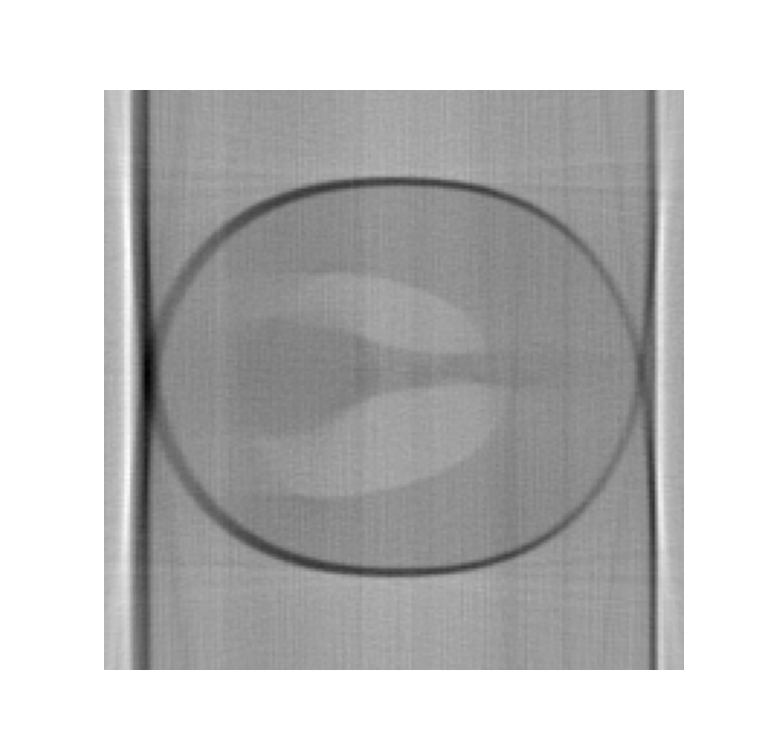
\includegraphics[width=\textwidth]{fbp_phantom_snr_20_unknown_angels.png}
      \caption{Noisy sinogram with \snry 20 dB reconstruction from GL estimated angles.}
      \label{fig:noisy_snr20_reco_unknown}
    \end{subfigure}\hfill
    \begin{subfigure}[t]{0.3\textwidth}
      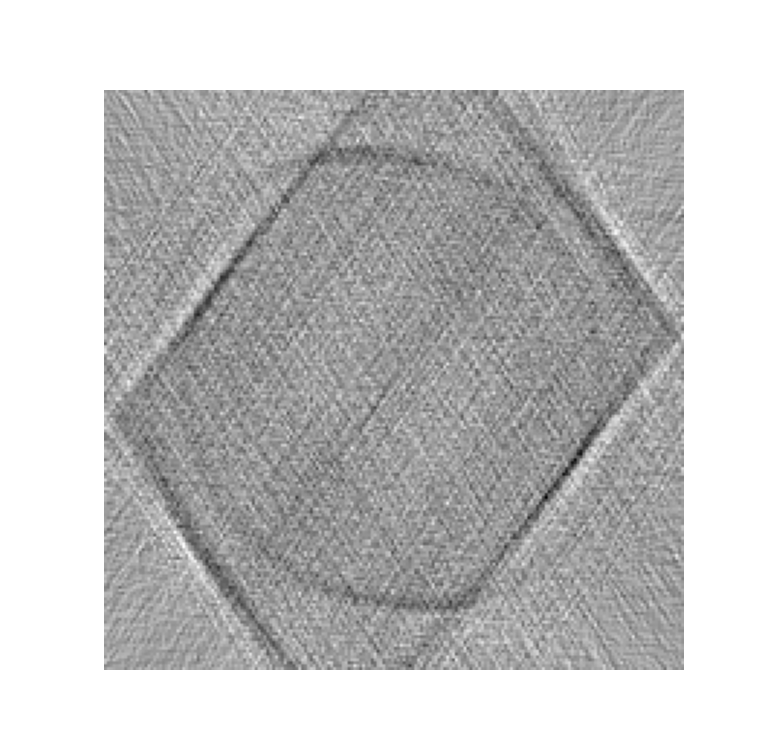
\includegraphics[width=\textwidth]{fbp_phantom_snr_0_unknown_angels.png}
      \caption{Noisy sinogram with \snry 0 dB reconstruction from GL estimated angles.}
      \label{fig:noisy_snr0_reco_unknown}
    \end{subfigure}

    \begin{subfigure}[t]{0.3\textwidth}
      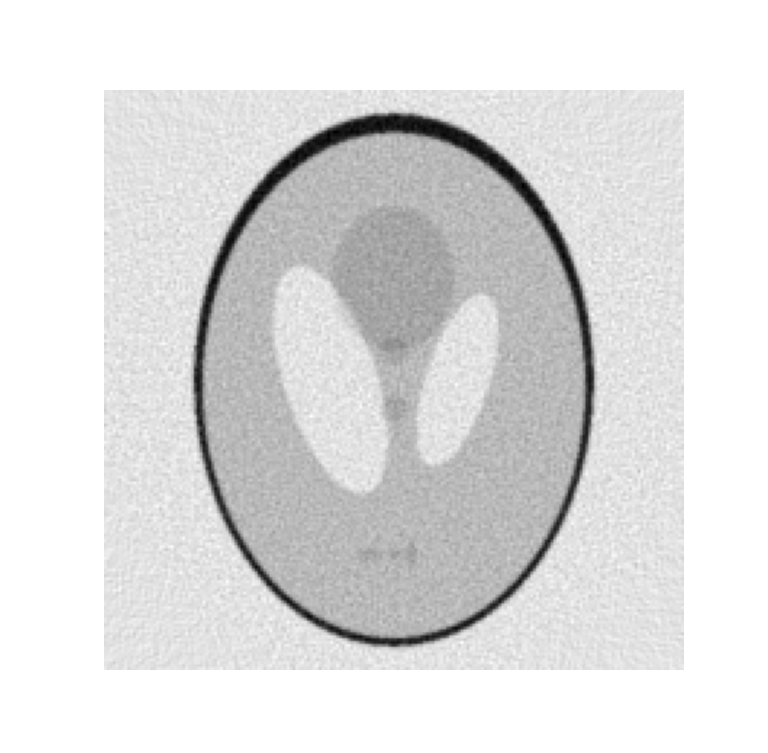
\includegraphics[width=\textwidth]{fbp_phantom_snr_20.png}
      \caption{Noisy sinogram with \snry 20 dB reconstruction from known angles.}
      \label{fig:noisy_snr20_reco_known}
    \end{subfigure}\hfill
    \begin{subfigure}[t]{0.3\textwidth}
      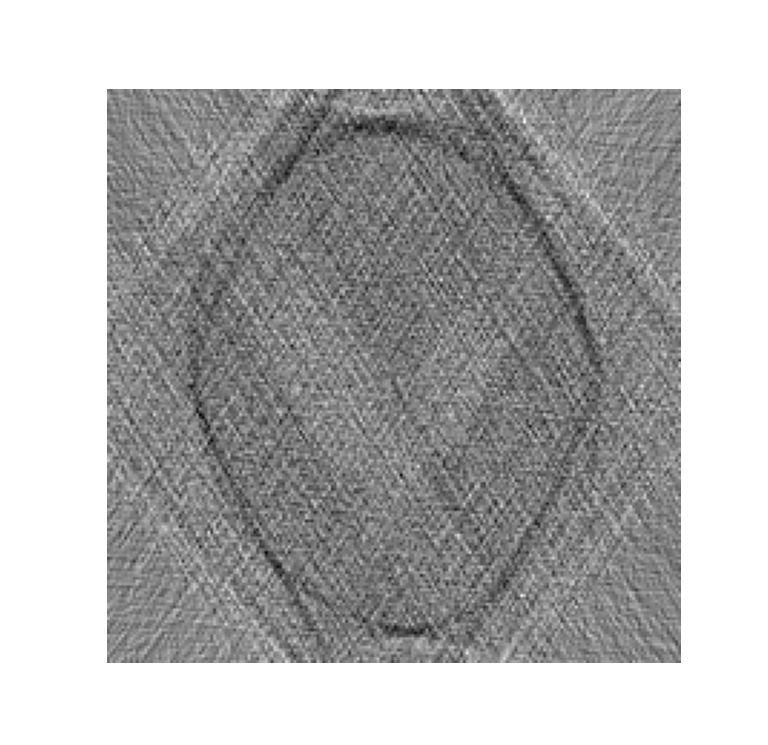
\includegraphics[width=\textwidth]{fbp_phantom_snr_0.png}
      \caption{Noisy sinogram with \snry 0 dB reconstruction from known angles.}
      \label{fig:noisy_snr0_reco_known}
    \end{subfigure}

    \caption{Shepp-Logan phantom sinogram GL eigenvectors}
    \label{fig:phantom_fbp_unknown_angles}
  \end{figure}

  Not only noise is reducing GL embedding quality, also $k$, number of observations 
  and observation dimension have an impact to the final result.
  Some further considerations are presented in Section~\ref{sec:embedding_quality}.

  \begin{tcolorbox}[colback=red!5!white,colframe=red!75!black]
    With the GL embedding of observations, angles can be approximated.
    Therefore, CT and cryo-EM problem can be solved for unknown angles, even tough the quality
    is slightly worse.
  \end{tcolorbox}

  \paragraph{Denoise observations:}
  As the quality of reconstruction is highly dependent on observations, it
  is expected to increase when the level of noise is decreased.
  Therefore, standard denoising methods like Block-matching and 3D filtering (BM3D) \cite{bm3d} or 
  non-local means \cite{noneLocalMean} could be used to denoise observations to get higher quality reconstructions.
  Both algorithms emerged from Signal Processing and are not operating on a graph structure. 
  But, they use a neighborhood for averaging, which shows great potential for graph 
  as a data structure for denoising, as graphs can represent neighborhoods really well.
  BM3D is considered the state-of-the-art denoising algorithm, before algorithms emerged from Deep Learning.
  Therefore, it will be used as a baseline algorithm in the practical part.
  Further, as illustrated with the GL embedding, graphs can restore information with a suitable prior,
  such as angles are uniformly sampled. 

  In this Thesis, 

\section{Graph Denoising}
\textit{Graph Denoising} is not a common term in literature.
In the current chapter, a way of constructing a k-NN graph from observations was introduced.
Moreover, the underlying true graph was found by computing the GL embedding, which is a circle or a sphere.
Therefore, our constructed graph from observations can be considered a noisy graph, 
as observations are noisy. 
As a consequence, the constructed noisy graph has some missing and additional edges compared to the true graph.
The goal of Graph Denoising is to estimate the original graph $G$ from a given noisy graph $G_0$.
In other words, noisy graph $G_0$ will be denoised.
This is my definition for Graph Denoising, which is rather related to signal or image denoising.
Reconstruction of a true signal given noisy observation signal is done via averaging, that can be performed

For every noisy graph there exists an original graph $G = \langle V,E \rangle$.
The noisy graph $G_0$ can further be defined as $G_0 = \langle V, E_0 \rangle$,  
 where $E_0 = E \setminus  E^{-}_0 \cup  E^{+}_0$ with $E^{-}_0 \subseteq E$ and $E^{+}_0 \cap E = \emptyset$.

$G_0$ consists of same nodes $V$ as original graph $G$. 
From $E$ some edges are removed (denoted by $E^{-}_0$) and some are added
(denoted by $E^{+}_0$), which results in edges $E_0$.

\paragraph{Connection to link prediction:}
Link prediction is a common task in Graph Learning. 
The goal is to predict existence of a link between two nodes.
The task can be formulated as a missing value estimation task. A model $M_p$ is learned
from a given set of observed edges. The model finally maps links to probabilities
$M_p : E^{\prime} \rightarrow [0,1]$ where $E^{\prime}$ is the set of potential links.

Further, $U$ determines the set of all possible edges of $G$, therefore $E \subseteq U$.
Clearly, Graph Denoising can be seen as a link prediction problem.
The difference is, that in link prediction a model from a set of observed links is learned
$E^{\prime} \subseteq E$ and in Graph Denoising model is learned from 
$E^{\prime} \subseteq U$. 
Link prediction problems are a subset of graph denoising problems.

\section{Graph Deep Learning}
\label{sec:graph_depp_learning}
Graph Denoising can be seen as a way of link predication. 
The state-of-the-art methods for solving link prediction are \textit{Graph Deep Learning} approaches.
With Graph Neural Networks (GNN)~\cite{GNN} the framework
for neural networks with graphs has been established. 

Using Graph Convolutional Networks (GCN)~\cite{GCN} for graph feature extraction is a popular way. 
With GCN a new feature representation is iteratively learned for node features (edge features are not considered).
It can be seen as an averaging of nodes over their neighborhood where all neighbors get the same weight combined with some non-linear activation (e.g. ReLu). 
To consider the node itself in averaging, \citet{GCN} applies the so-called "Renormalization trick", where self-loops are added to the 
adjacency matrix and after every layer, a normalization step is applied. 
The topology of the graph will not be adjusted during the learning process.

Simple Graph Convolutional Network~\cite{simpleGCN} proposed a simplified version of GCN.
They could verify their hypothesis that GCN is dominated by local averaging step and non-linear 
activation function between layers do not contribute too much to the success of GCN. 
Therefore, it can be seen as a way of power iteration\footnote{For more details see \ref{sec:powerIterations}}
over the adjacency matrix with normalization in every layer.
\citet{dynamicGCN} proposed an extension to GCN by not operating on the same graph in every layer but adopting
underlying graph topology layer by layer.
Graph Attention Networks (GAT) \cite{GAT} extended the concept of GCN with attention where not
all neighboring nodes get the same weight (attention).
Again, topology of the graph will not change but weighted averaging over the neighborhood 
will be computed and this is what in denoising is a good idea.
